\documentclass{standalone}
% preamble: usepackage, etc.

\begin{document}
\chapter{The Capability of Convolution Neural Network}
\label{Chapter3}

For diverse applications, several deep learning algorithms have been thoroughly examined, allowing for pattern and attribute understanding for the interpretation of both basic and complex representations. In the field of machine vision and learning, substantial advancements have recently been made. The convolution Neural Network (CNN) has advanced into a strong tool for perceptual image processing and pattern understanding. The CNN framework effectively captures distinctive insights using learnable attributes via convolutions by mimicking the human visual brain. Similarly, wavelet convolution Neural Networks' ability to learn both spatial and spectral details from sequential data like signal and image has increased efficiency and made significant contributions to tasks like disease diagnosis, machine fault diagnosis, biometric authentication and verification, and so on. As a result, both CNN and wavelet multi-resolution analysis have been coupled in order to produce meaningful visual interpretation. This is mostly the combination of machine vision and wavelet function algorithms.



\textbf{\section{A Case Study of COVID-19 Diagnosis}}

Towards the end of the last quarter of 2019, a new variant of SARS known as coronavirus (COVID-19) was first discovered in Wuhan city of China and ever since then, it has spread across the globe infecting over 177 million people and leading to more than 3.8 million deaths [1] and [2]. Due to the time it takes to develop a vaccine for the COVID-19 disease, timely diagnosis is of great necessity for prompt isolation and care for infected people in order to curb the wide spread of human-to-human transmission.

%\begin{figure*}[t!]
%\centering
%\includegraphics[scale=0.2]{pic/C3/c3_p1-1}
%\caption{The proposed COVID-Neurowavelet.}
%\label{fig:c3_p1-1}
%\end{figure*}

The World Health Organization has recommended some standard laboratory procedures for the diagnosis of COVID-19 of which the Reverse Transcription polymerase Chain Reaction (RT-PCR) is regarded as the gold standard [3] and [4]. One major bottleneck of RT-PCR is the low positive rate reported to be around 60\% for swab samples. This may undoubtedly result to misdiagnosis of patients which may further spread the disease to a large healthy population [5]. Chest radiography such as chest x-ray and chest tomography offer timely and easy way to diagnose pneumonia diseases [6]. 

%\begin{figure*}[t!]
%\centering
%\includegraphics[scale=0.4]{pic/C3/c3_p1-2}
%\caption{Chest X-ray images of the various pneumonia related  diseases including COVID-19  from COVID-CXR-12.}
%\label{fig:c3_p1-2}
%\end{figure*}

Image-based diagnosis of COVID-19 has been reported in literature to have high sensitivity [7]-[13]. COVID-19 radiography contains some subtle abnormalities that are difficult to interpret except for expert radiologists. Considering the ratio of the limited number of expert radiologists to the increasing number of infection cases, it is obvious that the margin is extremely huge therefore a fast method for detecting such subtle abnormalities can boost the screening procedures and improve timely diagnosis with satisfactory accuracy. Deep learning approach offers huge potential for solving such problem however, due to insufficient dataset, these models could perform poorly [3]. 

\begin{table}[]
%\scriptsize
\centering
\caption{Description of COVID-CXR-12 dataset showing number of images per category.}
\begin{tabular}{lllll}

\toprule
\textbf{\multicolumn{1}{l}{Dataset}} & \textbf{\multicolumn{1}{l}{Training set}} & \textbf{\multicolumn{1}{l}{Validation set}} & \textbf{\multicolumn{1}{l}{Test set}} & \textbf{\multicolumn{1}{l}{Total}} \\ \hline
\midrule
Atelectasis                   & 113                               & 32                                  & 17                            & 162                        \\
Bacteria                      & 113                               & 32                                  & 17                            & 162                        \\
Cardiomegaly                  & 133                               & 32                                  & 17                            & 162                        \\
Consolidation                 & 113                               & 32                                  & 17                            & 162                        \\
COVID-19                      & 113                               & 32                                  & 17                            & 162                        \\
Effusion                      & 113                               & 32                                  & 17                            & 162                        \\
Healthy                       & 113                               & 32                                  & 17                            & 162                        \\
Infiltration                  & 113                               & 32                                  & 17                            & 162                        \\
Mass                          & 113                               & 32                                  & 17                            & 162                        \\
Nodule                        & 113                               & 32                                  & 17                            & 162                        \\
Pneumothorax                  & 113                               & 32                                  & 17                            & 162                        \\
Virus                         & 113                               & 32                                  & 17                            & 162                        \\ \hline
\multicolumn{1}{l}{Total}   & \multicolumn{1}{l}{1,356}        & \multicolumn{1}{l}{384}            & \multicolumn{1}{l}{204}      & \multicolumn{1}{l}{}      \\ \hline 
\bottomrule
\end{tabular}
\label{tab1}
\end{table}

Unlike most literature that utilized stand-alone deep learning models which often perform poorly in extraction spatial details between images of close similarities [17], [18], we incorporated wavelet transfer multi resolution analysis into convolution neural network which directly filter the images and predict COVID-19 disease from CXR images. Wavelet based convolution neural network have been reported to outperform stand-alone convolution neural networks (CNN) [19]-[25]. We trained our proposed model alongside 4 well-known pre-trained deep learning models which have reported great achievement in different task on our 12 class CXR dataset (called COVID-CXR-12) and investigate their performance for COVID-19 identification. Since the dataset is quite small to train the transfer learning model from scratch, we employed the strategy of data augmentation to increase the dataset by creating transform versions of the data as well as fine-tuning the last layer of the pre-trained model to train on less labeled classes for which in our case is 12 classes. 

\begin{figure*}[t!]
\centering
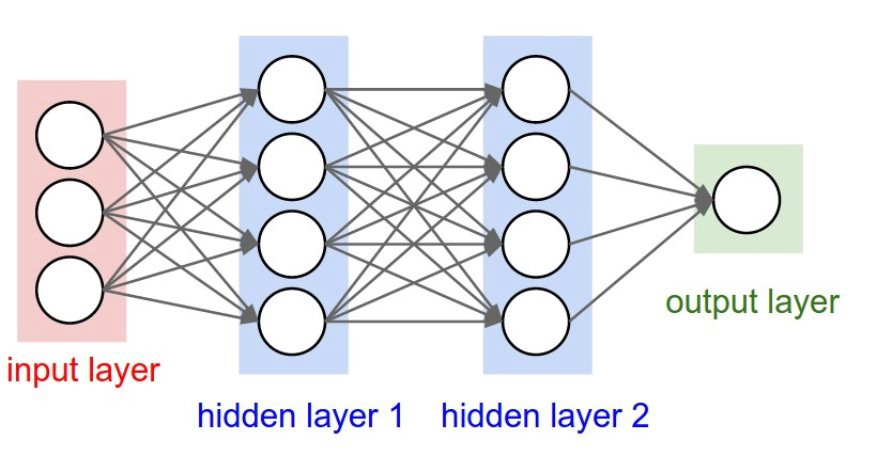
\includegraphics[scale=0.4]{pic/C3/c3_p1-3}
\caption{Illustration of  the discrete wavelet transform multi resolution analysis from 1-4 level decomposition using Haar wavelet function.}
\label{fig:c3_p1-3}
\end{figure*}

In as much as the dataset is quite small, we trained our proposed wavelet based convolution neural network (COVID-Neurowavelet) model from scratch. Several studies have reported the capability of wavelet convolution neural network for different image processing task [19], [21], and [24]. It is worth mentioning that the 4th level decomposition of our proposed model achieves quite a satisfactory result given the small amount of dataset. We believe that this work will serve as a benchmark for future works. 

\textbf{\subsection{The Proposed COVID-19 Neurowavelet}}

The proposed COVID-Neurowavelet is a wavelet convolution neural network for diagnosing COVID-19 from chest X-rays as shown in {Figure \ref{fig:c3_p1-1} }. The first three blocks have two CNN layers follow by batch normalization and ReLU activtion function whereas the fouth block has three CNN layer  follow by batch normalization and global average pool. Dropout of 0.5 is introduce in the fully connected layers for regularization. The branch  network consists of 6 convolutional layers for mapping the features of the wavelet inputs at each decomposition level into high dimensional features with samilar  filter size as the output features of each convolutional block to achieve channel-wise concatenation and dimentionality match. The proposed architecture consists of two parts.

The first part is the wavelet decomposition multi resolution analysis for image pre-processing and filtering while the second part is the convolution neural network for feature learning and classification. The first part tries to capture detailed features of the image and get rid of the noisy contents present in the image by means of a filtering technique. These high and low pass filters generate the detail and approximate components from the original image with the help of the wavelet and scaling function by down sampling with a scale factor of 2. The generated detail component is now the new input image fed to the convolution neural network for feature learning and classification. The generated approximate component is passed to the second level decomposition stage where it is further decomposed to generate a second level detail and approximate components. This process is repeated for four levels. 


The second part is subdivided into two pathways; the feature learning block and the concatenation block.  The feature learning block consists of 9 convolution layers where each convolution layer is followed by batch normalization and ReLU activation function. We did note utilize max pooling in our model rather we added global average pooling after the last convolution layers and a dropout of 50\% is added to each fully connected layer. The concatenation block consists of 3 channel-wise concatenation connected to 6 convolution layers. The first channel-wise concatenation is via a 1x1 convolution layer of 64 kernel size and second channel-wise concatenation is via two 1x1convolution layers of kernel size 64 and 128 respectively. The third channel-wise concatenation is via three  1x1  convolution layers of kernel size 64, 256 and 256 respectively. The model is trained on 20 epochs with batch of 16 and learning rate of 104 using Adam as the optimizer. The loss function adopted is the cross-entropy loss which ensures that the distance between the predicted score and the actual probability is minimized as define in {Equation \eqref{eq:1}}.

\begin{equation}
L_{CE}=-\sum_{i=1}^{N} {P_{i} log \ q_{i}}
\label{eq:1}
\end{equation}

where $P_i$ represents the actual class label and $q_i$ represents the predicted label. We adopted some evaluation metrics such as receiver operating characteristic (ROC) and precision-recall curves, area under curve (AUC), accuracy (ACC), sensitivity (SEN) and specificity (SPE). Details of the dataset utilized in the dissertation are described in subsequent headings.

\textbf{\subsection{Experiment Results}}

COVID-CXR-12 dataset is made up chest X-ray images collected from two open source dataset. We collected COVID-19 dataset from [14]. This dataset is a mixture of CT and CXR images and contains 250 CXR of COVID-19. It is important to mention that all our COVID-19 CXR is collected from this dataset. After cleaning and sorting, we arrived at a total of 162 scans of COVID-19 CXR based on the fact that only the images with observable radiographic signs are kept while every other CXR are discarded. Since the dataset repository consists of only COVID-19 and Non-COVID-19 images, we collected additional CXR of other pneumonia diseases from [15] to make up for the 12 classes. NIH dataset consists of 10,000 chest X-rays of pneumonia disease and 4,999 CXR scans of healthy patients from which we collected 162 images from each data class after thorough sorting. Table I give the number of images in COVID-CXR-12 including training, validation and test whereas Figure 2 shows the images from COVID-CXR-12.


\begin{table}[]
%\scriptsize
\centering
\caption{classification results of our proposed COVID-19 neurowavelet.}
\begin{tabular}{lllll}
\toprule
\multicolumn{1}{l}{Dataset}                     & \multicolumn{1}{l}{Accuracy (\%)} & \multicolumn{1}{l}{AUC (\%)} & \multicolumn{1}{l}{Specificity (\%)} & \multicolumn{1}{l}{Sensitivity (\%)} \\\hline
\midrule
CNN   without wavelet                             & 88                                 & 87                            & 89                                    & 90                                    \\
CNN +   1-level decomposition                     & 95                                 & 94                            & 94                                    & 95                                    \\
CNN +   2-level decomposition                     & 96                                 & 96                            & 96                                    & 97                                    \\
CNN +   3-level decomposition                     & 98                                 & 98                            & 97                                    & 99                                    \\ \hline
\multicolumn{1}{l}{CNN + 4-level decomposition} & \multicolumn{1}{l}{99}            & \multicolumn{1}{l}{99}       & \multicolumn{1}{l}{99}               & \multicolumn{1}{l}{100}  \\ \hline
\bottomrule
\end{tabular}
\label{tab2}
\end{table}

To perform a 2D discrete wavelet transform (DWT) as illustrated in Figure 3a, the images are first passed via a half-band high and low pass filters. After the filtering process, the images are sub sampled into detail and approximate coefficients using scaling and wavelet function. The images are scaled to a frequency bandwidth of π⁄2 radian using Haar wavelet function. Since the detail coefficient is characterized mainly with low frequency components, it is therefore concatenated via the channel-wise as input to the CNN block. Instead of eliminating the approximate coefficient generated in the 1-level decomposition stage simply because it consists mainly of high frequency components, it is therefore further decomposed to generate detail and approximate coefficients after undergoing the same filtering process as mentioned in the first level decomposition stage as shown in Figure 3b. The low frequency detail coefficient is concatenated via the channel-wise as input to the CNN block. 

The same process is repeated for the 3-level decomposition stage in which the approximate is further decomposed to generate a 3-level detail and approximate coefficients as seen in Figure 3c. The low frequency detail coefficient is concatenated via the channel-wise as input to the CNN block. 

Finally, as seen in Figure 3d, the further decomposition of the 3-level approximate coefficient generates a new set of detail and approximate coefficients that are aggregated as single input and concatenated via channel-wise to the CNN block. 

\textbf{\subsection{Discussion}}

This section reports the performance of COVID-Neurowavelet model on COVID-CXR-12. More importantly, we compared our proposed model in two categories: 1) we trained 4 famous pre-trained deep learning models on COVID-CXR-12 and compare their results with ours. 2) We compared our result with other image-based COVID-19 state-of-the-art models. Several studies have shown that deep learning models exhibit different converging patterns due to variations in data type and quantity. To analyze the claim, we conducted the first experiment by training our proposed CNN architecture from scratch without integrating discrete wavelet transform. From our analysis, the model achieves 88\% accuracy, 90\% sensitivity, and 89\% specificity as shown in Table II. In our second experiment, we integrated 1-level DWT decomposition into our proposed CNN architecture and the performance significantly increased at a margin of 5-6\%. The model achieves 95\% accuracy, 95\% sensitivity, and 94\% specificity as shown in Table II. From all indications, DWT has the capability to influence the convergence behavior of deep learning model during training. In our third experiment, we considered a 2-level DWT decomposition and obtained a better performance of 96\% accuracy, 97\% sensitivity, and 96\% specificity as illustrated in Table II. 

Further decomposition of the discrete wavelet transforms at the 3-level significantly increase the performance of the model by a margin of 2\% across the evaluation metrics achieving 98.5\% accuracy, 97\% specificity, and 99\% sensitivity. It is worth mentioning that our proposed model converges smoothly and fast as the decomposition level increases. The 4-level DWT decomposition shows a gentle increment in the model performance by a margin of 1\% achieving 99\% accuracy, 99\% specificity, and 100\% sensitivity as seen in Table II. Figure 4 shows the ROC curves of all the decomposition levels and their AUC values. Figure 5 presents the precision-recall curves for all decomposition levels and their average precision scores. 

\begin{table}[]
%\scriptsize
\centering
\caption{Comparison of the proposed model with state-of-the-art image based covid-19 diagnosis models.}
\begin{tabular}{lllll}
\toprule
\textbf{\multicolumn{1}{l}{Literature}}   & \textbf{\multicolumn{1}{l}{Accuracy   (\%)}} & \textbf{\multicolumn{1}{l}{Sensitivity   (\%)}} & \textbf{\multicolumn{1}{l}{Specificity   (\%)}} & \textbf{\multicolumn{1}{l}{AUC (\%)}} \\ \hline
\midrule
Wang et al {[}28{]}                    & 92.3                                 & 90.4                                    & 89.5                                    & 91.5                          \\
Shi et al {[}29{]}                     & 87.9                                 & 90.7                                    & 83.3                                    & 89.5                          \\
Jin et al {[}13{]}                     & 96.5                                 & 94.5                                    & 92.8                                    & 89.4                          \\
Xu et al {[}3{]}                       & 86.7                                 & 87.9                                    & 90.7                                    & 91.5                          \\
Wang et al {[}4{]}                     & 82.9                                 & 85.9                                    & 89.4                                    & 88.7                          \\
Barstugan et al {[}26{]}               & 90.7                                 & 91.8                                    & 92.3                                    & 95.7                          \\ \hline
\multicolumn{1}{l}{Ours   (4-level)} & \multicolumn{1}{l}{99}              & \multicolumn{1}{l}{100}                & \multicolumn{1}{l}{99}                 & \multicolumn{1}{l}{99}       \\ \hline
\bottomrule
\end{tabular}
\label{tab3}
\end{table}

The 4-level decomposition obtained the best results across all the metrics. The reason for the steady and fast convergence of our proposed model can be attributed to the fact that wavelet reduces the training load of learning the network layers that reconstruct the low frequency information. It is important to mention that the steady increase in performance of our model is as a result of the ability of wavelet to work on transform domain data in order to capture more structural details in the images to eliminate artifacts. On the bases of fair comparison, we trained 4 famous ImageNet pre-trained models on COVID-CXR-12 by fine-tuning the last layer to correspond to the number of classes in our dataset. Table IV reports the performance of these models. Figure 6 presents the ROC curves of the pre-trained models with their AUC values. 


More so, the average precision score for each pre-trained model is presented in the precision-recall curves illustrated in Figure 7. It is worth mentioning that the low performance of these pre-trained models is attributed to the size of the dataset and the complexity of the networks. At some point, these models encountered exploding and vanishing gradient problem where they could no longer learn anymore due to over saturation. This bottleneck presents our proposed model as an alternative solution to COVID-19 AI-based system in the face of data scarcity. Table III presents comparison results of previous state-of-the-art COVID-19 diagnostic models with our proposed model.

\textbf{\subsection{Comparison}}

We will present some state-of-the-art results by comparing them with our proposed model. Barstugan et al [26] proposed a technique of incorporating machine learning algorithm into deep learning network for the classification of COVID-19 from CT exams. Wang et al [27] and Xu et la [3] suggested an interesting work of detecting COVID-19 from CXR using deep learning model with few indicators. Jin et al [13] suggested a logistic regression technique to detect COVID-19. Li et al [10] proposed a dual CNN method to detect COVID-19 using CT exams. Shi et al [12] suggested a method of random forest to identify COVID-19. The findings of the aforementioned methods are presented in Table III

\begin{table}[]
%\scriptsize
\centering
\caption{Performance comparison of selected deep learning models. From all indications, the proposed wavelet integrated neural network exhibits the highest score.}
\begin{tabular}{lllll}
\toprule
\textbf{\multicolumn{1}{l}{Famous   Network}} & \textbf{\multicolumn{1}{l}{Accuracy (\%)}} & \textbf{\multicolumn{1}{l}{AUC (\%)}} & \textbf{\multicolumn{1}{l}{Specificity (\%)}} & \textbf{\multicolumn{1}{l}{Sensitivity (\%)}} \\ \hline
\midrule
VGG16                                  & 83.4                               & 89.8                          & 90.1                                  & 90.2                                  \\
Inception V3                           & 91.5                               & 84.6                          & 85.6                                  & 91.5                                  \\
ResNet50                               & 94.5                               & 87.5                          & 88.5                                  & 95.3                                  \\
VGG19                                  & 94.7                               & 86.8                          & 86.9                                  & 97.5                                  \\ \hline
\multicolumn{1}{l}{Ours   (4-level)} & \multicolumn{1}{l}{99}            & \multicolumn{1}{l}{99}       & \multicolumn{1}{l}{99}               & \multicolumn{1}{l}{100}              \\\hline 
\bottomrule
\end{tabular}
\label{tab4}
\end{table}

Reference [16] claimed that human-centered detection method of COVID-19 by radiologist using CXR could achieve high sensitivity but with very low specificity around 30\%. This low specificity usually amount to increase in false positive prediction which eventually leads to wrongly administered treatment and expense. It is obvious that our proposed model, COVID-Neurowavelet achieves a very high specificity of 99\% for the 4-level decomposition which can be considered to help expert radiologist to mitigate the reported cases of false positive. More so, the reported result in terms of Receiver Operating Characteristic (ROC) can assists expert radiologist form a balance between sensitivity and specificity.

In conclusion, it is imperative to make some commendable remarks on COVID-Neurowavelet computational cost and model complexity. By introducing wavelet transform, the use of max pool at each convolution block was eliminated thereby reducing model complexity and computational time. Another interesting advantage of our COVID-Neurowavelet is the ability to reduce noise in the input images as we concatenate the features of the generated detail coefficients and the output features of the previous convolution layer at each level of decomposition to every convolution block via 1x1convolution layer. Talking about computational cost, our model was trained for 16 minutes on NVIDIA GTX 1080. We adopted Keras framework for implementing our architecture. The model complexity of the proposed model is far reduced due to less training parameters compared to previous state-of-the-art models.

\textbf{\subsection{Conclusion}}

Our study presents the capability of multi resolution analysis for detecting COVID-19 CXR by investigating the effect of discrete wavelet transform decomposition up to 4-levels. At each decomposition level, the wavelet sub-bands are the inputs to the CNN. We put together a dataset of 1,944 CXR images of 12 classes called COVID-CXR-12 collected from two open source datasets. We trained our proposed model COVID-Neurowavelet on COVID-CXR-12 alongside other famous ImageNet pre-trained models. COVID-Neurowavelet is significantly cost-effective in terms of the number of parameters compared to the pre-trained and other state-of-the-art models and yet obtains state-of-the-art results. 


\end{document}
